% !TEX spellcheck = en-GB
\documentclass[onecolumn,notitlepage,superscriptaddress, nofootinbib,nobibnotes, aps,prd,10pt]{revtex4-1}% secnumarabic, 
\usepackage{amsmath,amssymb, fp}  
\usepackage{xcolor}  
\usepackage{soul} 
\usepackage{booktabs}
\usepackage{physics}
%\allowdisplaybreaks

\newcommand{\s}[2]{#1^{(#2)}}
%\definecolor{linkcolor}{RGB}{150,50,60}  
%\definecolor{linkcolor}{RGB}{9,82,60}  %green
%\definecolor{linkcolor}{RGB}{18,140,126}  %teal green
\definecolor{linkcolor}{RGB}{7,94,84}  %teal dark green
%\definecolor{linkcolor}{RGB}{207,80,0}  %orange
\usepackage[	colorlinks=true,    	
			pdfstartview=FitV,
			linkcolor= linkcolor,
			citecolor= linkcolor,
			urlcolor= linkcolor,
			linktoc=page,
			hyperindex=true,
			hyperfigures=true,  
			breaklinks=true]
			{hyperref}
%\hypersetup{colorlinks=true,	
%			pdfstartview=FitV,  
%			linkcolor= linkcolor,
%			citecolor= linkcolor,
%			urlcolor= linkcolor,
%			linktoc=page,
%			hyperindex=true,
%			hyperfigures=true}
\usepackage{dblfloatfix}    
\usepackage{balance} 
\usepackage{lastpage}  
\usepackage{mathtools}
\usepackage{epsfig,rotating,pifont}
\usepackage{graphicx}
\graphicspath{{./figures/}}	
%\usepackage{wrapfig}
%\usepackage{caption}
%\usepackage{subcaption}
\usepackage[caption=false]{subfig}
\usepackage{placeins}
%\usepackage[hypcap=true]{caption}
%\captionsetup{justification=justified, format=plain}
%\usepackage{relsize}
%\usepackage{bbold}

%\usepackage{dsfont}

%\usepackage{pifont, indentfirst, dsfont, relsize}
\usepackage{ragged2e} 
\usepackage{etoolbox}
\usepackage{changepage}   % for the adjustwidth environment
\usepackage{pgfplots}
\usetikzlibrary{pgfplots.groupplots}
\pgfplotsset{compat=1.3}
\usepackage{tikz}  
\usetikzlibrary{arrows,shapes,positioning}
\usetikzlibrary{decorations.markings,decorations.pathmorphing,decorations.pathreplacing,decorations.text}
\usetikzlibrary{arrows,calc,patterns,shapes.geometric}
\usepackage{fancybox}
\usepackage{verbatim}
\usepackage{multirow}
\usepackage{titlesec}
%\usepackage[sort,compress]{cite}
%\usepackage[titletoc, title]{appendix}
%\usepackage{cite}
%\usepackage{authblk}
\newcommand{\revtex}{REV\TeX\ }
\newcommand{\classoption}[1]{\texttt{#1}}
\newcommand{\macro}[1]{\texttt{\textbackslash#1}}
\newcommand{\m}[1]{\macro{#1}}
\newcommand{\env}[1]{\texttt{#1}}
\setlength{\textheight}{9.5in}

\newsavebox\CBox 
\def\textBF#1{\sbox\CBox{#1}\resizebox{1\wd\CBox}{0.97\ht\CBox}{\textbf{#1}}}

%\DeclareMathSizes{10}{10}{7}{5}
%\DeclareMathSizes{<current font size>}{<size for textstyle>}{<size for scriptstyle>}{<size for scriptscriptsize>} %default: 10 10 7 5

%\usepackage{exscale}
%\usepackage{array,multicol}
%\usepackage{afterpage,float,flafter}
%\usepackage{epsfig,rotating,pifont}

%\usepackage[sort,compress]{cite}

\def\beq{\begin{eqnarray}}
\def\eeq{\end{eqnarray}}
\def\m{M_*}
%\def\msm{M_{\rm SM}}
\def\mpl{M_{\rm Pl}}
\def\e{{\epsilon}}
\def\v{{\cal V}}
\def\bo{{\nabla^2}}
\def\fu{{\cal F}}


%\usepackage[notref,notcite]{showkeys}
\def\const{\mbox{const}}
\def\e{{\rm e}}
\def\a{\alpha}
\def\b{\beta}
\def\eps{\epsilon}
\def\d{\partial}
\def\l{\left(}
\def\r{\right)}
\def\la{\langle }
\def\ra{\rangle }
\def\o{\over}
\def\ba{\bar{a}}
\def\bb{\bar{b}}
\def\lb{\label}
\def\om{\Omega}
\def\M{\mathcal{M}}
\def\H{\mathcal{H}}
\def\A{\mathcal{A}}
\def\B{\mathcal{B}}
\def\O{\mathcal{O}}
\def\P{\mathcal{P}}
\def\E{\mathcal{E}}
\def\DM{\partial\mathcal{M}}
\def\pip{\Pi_+}
\def\pim{\Pi_-}
\def\Kh{\hat{K}}
\def\Db{\mathring{\nabla}}
\def\Boxb{\mathring{\Box}}
\def\D{\nabla}
\def\C{\mathcal{C}}
\def\cca{\mathfrak{a}}
\def\K{{|\hspace{-2pt}<}}
\newcommand{\balancedVPhantom}[1]{% gives minimum vertical size
$\mathsurround=0pt \vcenter{\hrule width0pt height #1}$\ignorespaces}


%%%%%%%%%%%%%%%%%%%%% NDV's %%%%%%%%%%%%%%%%%%%%%%%%%%%%%%%
\newcommand{\spt}{s}     % starting proper time
\newcommand{\apt}{\sigma}   % auxiliary proper time


\newcommand{\sco}{\epsilon_{\spt}}              % starting cut-off
\newcommand{\aco}{\varepsilon_{\apt}}             % auxiliary cut-off


\newcommand{\Cont}[1] {\,^{#1}\P}               % Contour
\newcommand{\CMdim}[1]    {{\mathfrak{M}^{#1}}} % Curvature Mass Dimension (Background dimensionality)

%\newcommand{\pBox}{{|\Box|}}
\newcommand{\pB}{{\Delta}}

\newcommand{\pBt}{{\Delta_t}}
\newcommand{\pBx}{{\Delta_x}}

\newcommand{\Nl}{\mathrm{N}}      % Lapse function in ADM decomposition
%\newcommand{\Nsh}{N}             % Shift function in ADM decomposition   -- already defined

%\newcommand{\Tr}{\mathrm{Tr}\hspace{1pt}}            % already defined
\newcommand{\ad}{{\mathrm{ad}}}

%##########%   %###########% HK.Commands.tex %############%   %##############%
 %% Indices of the first type

\newcommand{\za}{{\alpha}}   %a
\newcommand{\zb}{{\beta}}    %b
\newcommand{\zc}{{\gamma}}   %c
\newcommand{\zd}{{\delta}}   %d
\newcommand{\zk}{{\kappa}}   %k
\newcommand{\zl}{{\lambda}}  %l
\newcommand{\zm}{{\mu}}      %m
\newcommand{\zn}{{\nu}}      %n
\newcommand{\zp}{{\pi}}     %p
\newcommand{\zr}{{\rho}}     %r
\newcommand{\zs}{{\sigma}}   %s

\newcommand{\z}{{\phantom{\za}}}

 %% Indices of the 2 type (large)

\newcommand{\ZA}{{\scriptscriptstyle{\!A}}}   %a
\newcommand{\ZB}{{\scriptscriptstyle{\!B}}}   %b
\newcommand{\ZC}{{\scriptscriptstyle{\!C}}}   %c
\newcommand{\ZD}{{\scriptscriptstyle{\!D}}}   %d
\newcommand{\ZE}{{\scriptscriptstyle{E}}}   %e
\newcommand{\ZF}{{\scriptscriptstyle{F}}}   %f
\newcommand{\ZK}{{\scriptscriptstyle{\!K}}}   %k
\newcommand{\ZL}{{\scriptscriptstyle{\!L}}}   %l
\newcommand{\ZM}{{\scriptscriptstyle{\!M}}}   %m
\newcommand{\ZN}{{\scriptscriptstyle{\!N}}}   %n
\newcommand{\ZP}{{\scriptscriptstyle{P}}}   %p
\newcommand{\ZQ}{{\scriptscriptstyle{Q}}}   %q
\newcommand{\ZR}{{\scriptscriptstyle{R}}}   %r
\newcommand{\ZS}{{\scriptscriptstyle{S}}}   %s

\newcommand{\Z}{{\phantom{\scriptscriptstyle{\ZA}}}}

\newcommand{\R}{{\mathbb R}} % Real Numbers  % amssymb
\newcommand{\N}{{\mathbb N}} % Natural Numbers  %{{\mathbb N}^{*}} 1,2,3,


\newcommand{\DeltaF}{\mathrm{\delta}}  % Dirac delta-function
\newcommand{\ThetaF}{\mathrm{\theta}}  % Heviside theta-function
\newcommand{\eg}{{\it e.g.,}\ }
\newcommand{\ie}{{\it i.e.,}\ }

\newcommand{\sign}{\mathop{sgn}\nolimits} % LaTeX  %% ?????????, ???. 47


 % Gamma-function:
 \newcommand{\GammaF}[1] {{\ensuremath{\mathchoice%
      {\,\mathrm{\Gamma}{\textstyle\left(#1\right)}}%        display math mode
      {\,\mathrm{\Gamma}{\textstyle\big(#1\big)}}%        in-line math mode
      {\,\mathrm{\Gamma}{\scriptstyle(#1)}}%       scriptstyle
      {\,\mathrm{\Gamma}{\scriptscriptstyle\left(#1\right)}} }}}%    scriptscriptstyle



\newcommand{\fracd}[2]{{\displaystyle\frac{#1}{#2}}}
\newcommand{\fract}[2]{{\textstyle\frac{#1}{#2}}}
\newcommand{\fracs}[2]{{\scriptstyle\frac{#1}{#2}}}
\newcommand{\fracss}[2]{{\scriptscriptstyle\frac{#1}{#2}}}

%%%%%%%%%%%%%%%%%%%%%%%%% End NDV's %%%%%%%%%%%%%%%%%%%%%%%%%%%%%%%%%%%%%%%%

%\newcommand{\be}{\begin{equation}}
%\newcommand{\ee}{\end{equation}}
%\newcommand{\bea}{\begin{eqnarray}}
%\newcommand{\eea}{\end{eqnarray}}
%\newcommand{\bg}{\begin{gather}}
%\newcommand{\eg}{\end{gather}}

\newcommand{\bt}{\beta}
\newcommand{\bseq}{\begin{subequations}}
\newcommand{\eseq}{\end{subequations}}
\newcommand{\tg}{\mathop{\rm tg}\nolimits}
\newcommand{\arctg}{\mathop{\rm arctg}\nolimits}
\renewcommand{\tanh}{\mathop{\rm th}\nolimits}
\newcommand{\ch}{\mathop{\rm ch}\nolimits}
\newcommand{\sh}{\mathop{\rm sh}\nolimits}
\renewcommand{\ln}{\mathop{\rm ln}\nolimits}
\newcommand{\sm}[1]{{\scriptscriptstyle \rm #1}}
%\newcommand{\Tr}{{\rm Tr}}
\renewcommand{\Im}{\mathop{\rm Im}\nolimits}
\renewcommand{\Re}{\mathop{\rm Re}\nolimits}
\def\half{\frac{1}{2}}
\newcommand{\eq}[1]{(\ref{#1})}
\newcommand{\goe}{\gtrsim}
\newcommand{\loe}{\lesssim}
%\newcommand{\bra}[1]{\langle #1 |}
%\newcommand{\ket}[1]{| #1 \rangle}
\def\theenumi{(\alph{enumi})}
\def\tr{{\rm Tr}}
\def\r{\rho}
\def\be{\begin{eqnarray}}
\def\ee{\end{eqnarray}}
\def\lb{\label}
\def\K{{|\hspace{-2pt}<}}
\def\emi{{\scalebox{0.6}{{\rm EMI}}}}
\def\bemi{{\scalebox{0.6}{\rm bEMI}}}
\def\LFT{{\scalebox{0.6}{\rm LFT}}}
\def\LFT{{{z=2}}}
\def\dra{{\ra\hspace{-2pt}\ra}}
\def\dla{{\la\hspace{-2pt}\la}}
\def\n{\mathrm{n}}
\def\h{\mathfrak{h}}
\def\S{\mathcal{S}}
\def\nn{\nonumber}
\def\hs{\hspace{1pt}}
\def\hsm{\hspace{-1pt}}

\def\dd{\mathrm{d}}
\newcommand{\zbar}{\bar{z}}



\definecolor{Green}{RGB}{147,162,153}
\definecolor{Green2}{RGB}{26,148,49}
\definecolor{BrownL}{RGB}{173,143,103}
\definecolor{Red}{RGB}{210,83,60}
\definecolor{BrownD}{RGB}{114,96,86}
\definecolor{GreyD}{RGB}{76,90,106}
\definecolor{GreyB}{RGB}{128,141,160}
\definecolor{Maroon}{RGB}{121,70,61}
\definecolor{Blue}{RGB}{148,184,210}
\definecolor{Blue2}{RGB}{108,144,170}
\definecolor{Blue3}{RGB}{42, 107, 172}
\definecolor{BB}{RGB}{128,184,220}  
%\newcommand{\red}[1]{{\color{Red}#1}}
\newcommand{\red}[1]{#1}
\newcommand{\blue}[1]{\textbf{\color{Blue2}#1}}
\newcommand{\Blue}[1]{\textbf{\color{blue}#1}}
\newcommand{\grey}[1]{\textbf{\color{GreyB}#1}}
\newcommand{\brown}[1]{\textbf{\color{BrownL}#1}}
\newcommand{\maroon}[1]{\textbf{\color{Maroon}#1}}

\newsavebox\foobox
\newcommand\slbox[2]{%
  \FPdiv{\result}{#1}{57.296}% CONVERT deg TO rad
  \FPtan{\result}{\result}%
  \slantbox[\result]{#2}%
}%
\newcommand{\slantbox}[2][30]{%
        \scalebox{1}[.7]{\mbox{%
        \sbox{\foobox}{#2}%
        \hskip\wd\foobox
        \pdfsave
        \pdfsetmatrix{1 0 #1 1}%
        \llap{\usebox{\foobox}}%
        \pdfrestore
}}}
\newcommand\rotslant[3]{\rotatebox{#1}{\slbox{#2}{#3}}}

%%%%%%% Balance column appendix
%\makeatletter
%    \def\balanceissued{unbalanced}%flag to indicate if \balance has been used
%    \let\oldbibitem\bibitem
%    \def\bibitem{%
%        \ifnum\thepage=\lastpage@lastpage%
%            \expandafter\ifx\expandafter\relax\balanceissued\relax\else%
%                \balance%
%                \gdef\balanceissued{\relax}\fi%
%            \else\fi%
%        \oldbibitem}
%\makeatother
%%%%%%%%

\let\revappendix\appendix


%%%%%%%%%%%%%%%%%%%%%%%%%%%%%%%%%%%%%%%%%%%%%%%%%%%%%%%%%%%%%%%%%

\begin{document}


\title{General relativistic quantum mechanics: \\  \smallskip Action-Angle reparametrization invariance and $\omega_{\infty}$ symmetry}  

\author{Jibril Ben Achour}
\affiliation{Arnold Sommerfeld Center for Theoretical Physics, Munich, Germany}
\affiliation{Munich Center for Quantum Science and Technology, Germany}
\affiliation{Univ de Lyon, ENS de Lyon, Laboratoire de Physique, CNRS UMR 5672, Lyon 69007, France}
%\email{clement.berthiere@umontreal.ca}
\author{Alexander F. Jercher}
\affiliation{Arnold Sommerfeld Center for Theoretical Physics, Munich, Germany}
\affiliation{Munich Center for Quantum Science and Technology, Germany}
\affiliation{Theoretisch-Physikalisches Institut, Friedrich-Schiller-Universit\"{a}t Jena, Max-Wien-Platz 1, 07743 Jena, Germany, EU}
\author{Etera R. Livine}
\affiliation{Univ de Lyon, ENS de Lyon, Laboratoire de Physique, CNRS UMR 5672, Lyon 69007, France}



%\date{\today} 
 
\begin{abstract}\vspace{-1pt}
\begin{center}\textbf{\abstractname}\end{center}\vspace{-3pt} 
%



\vspace*{-8pt}
$\,$

%
\end{abstract}

\maketitle  

\makeatletter
%\def\l@subsubsection#1#2{}
\makeatother
\tableofcontents

\section{Introduction}

Quantizing gravity versus gravitizing the quantum\\
First step, understand how to relax the notion of space and time in quantum mechanics.
A preliminary step towards this goal: formulate mechanics in a covariant language, where time is no longer absolute: mechanics equipped with time reparametrization invariance.
Study the structure of this covariant mechanics: symmetry, charges and algebra towards quantization.

Literature, I stumbled across and that might be useful
\begin{itemize}
    \item \href{https://www.scirp.org/html/23892.html}{Any Hamiltonian System Is Locally Equivalent to a Free Particle}
    \item \href{https://sci-hub.ru/https://doi.org/10.1119/1.10618}{Canonical transformation to the free particle}
    \item We can always switch between $H$ and $T_0$ and thus have an interpretation of each diffeo in term of time reparametrization. There are three possibilities
    \begin{itemize}
    \item Gauge symmetry
    \be
    \tau \rightarrow f(\tau) \qquad S[T_0 ,H; \tilde{\tau}] = \int \dd{  \tilde{\tau} }H \frac{\dd{T_0}}{\dd{ \tilde{\tau}}} = \int \dd{ \tau }H \frac{\dd{T_0}}{\dd{ \tau}} = S[T_0 ,H; \tau]
    \ee
    \item Physical symmetry as reparametrization of initial conditions
    \item Physical symmetry as a field dependent time-reparametrization
    \end{itemize}
    \item Geodesic action in 1d space: coordinate $T_0$, lapse $g_{11} = N=H$
    \be
    S = \int \dd{\tau} \sqrt{g_{\mu\nu} \frac{\dd{ x^{\mu}}}{\dd{ \tau}} \frac{\dd{ x^{\nu}}}{\dd{ \tau} }} =  \int \dd{\tau} \sqrt{g_{11} \frac{\dd{ T_0}}{\dd{ \tau}} \frac{\dd{ T_0}}{\dd{ \tau} }} =  \int \dd{\tau} \sqrt{H^2 \frac{\dd{ T_0}}{\dd{ \tau}} \frac{\dd{ T_0}}{\dd{ \tau} }} =  \int \dd{\tau} H\frac{\dd{ T_0}}{\dd{ \tau}} 
    \ee
    \item $W_{\infty}$ charge algebra
    \item Quantum effect: two labels for the states
\end{itemize}

\newpage

\section{Covariant mechanics}

\subsection{Angle-action variables and time reparametrization invariance}

\subsection{A geometrical interpretation: geodesic flow in the space of motion}

Consider the geodesic action
    \be
    S = \int \dd{\tau} \sqrt{g_{\mu\nu} \frac{\dd{ x^{\mu}}}{\dd{ \tau}} \frac{\dd{ x^{\nu}}}{\dd{ \tau} }} 
    \ee
    on a 1d geometry coordinatized by $T_0$ .The line element is simply
    \be
    \dd s^2 = g_{T_0 T_0} \dd T^2_0 \qquad \text{with} \qquad g_{T_0 T_0} = H^2
    \ee
    where $H$ plays the role of the lapse function. It is then direct to see that this geodesic lagrangian reproduces exactly the previous lagrangian, i.e one has
    \be
    S = \int \dd{\tau} \sqrt{g_{\mu\nu} \frac{\dd{ x^{\mu}}}{\dd{ \tau}} \frac{\dd{ x^{\nu}}}{\dd{ \tau} }} =  \int \dd{\tau} \sqrt{g_{11} \frac{\dd{ T_0}}{\dd{ \tau}} \frac{\dd{ T_0}}{\dd{ \tau} }} =  \int \dd{\tau} \sqrt{H^2 \frac{\dd{ T_0}}{\dd{ \tau}} \frac{\dd{ T_0}}{\dd{ \tau} }} =  \int \dd{\tau} H\frac{\dd{ T_0}}{\dd{ \tau}} =  \int  H \dd{ T_0}
    \ee
    
    
    \section{Generally covariant mechanics}

\subsection{Infinite dimensional Noether symmetry and  $\text{\textbf{\textit{w}}}_{\mathbf{\infty}}$-algebra}\label{sec:Hidden Noether symmetry}



For a $1$-dimensional mechanical system characterized by position and conjugate momentum $(q,p)$, the Hamilton-Jacobi formalism~\cite{Goldstein1980} allows to construct a canonical transformation $(q,p)\rightarrow (T_0,H)$ to a set of variables $(T_0,H)$ for which the new Hamiltonian vanishes,  $K(T_0,H) = 0$. Thus, the new variables are constants of motion, i.e. $\dot{T}_0 = \dot{H} = 0$. The corresponding action functional takes the form
%
\begin{equation}\label{eq:action}
S[T_0,H] = \int H\dd{T}_0 = \int H\dot{T}_0\dd{t}.
\end{equation}
%
As the example of the harmonic oscillator in Sec.~\ref{sec:Example} shows, the variable $T_0$ can be understood as evolving constant of motion, $T_0(q,p,t)= T(q,p)-t$ that characterizes the initial time, where $T(q,p)$ is an explicitly phase space-dependent function conjugate to the Hamiltonian $H(q,p)$. 

Each set of initial values $(T_0,H)$ characterizes a solution to the equations of motion. Therefore, the canonical transformation described here provides a map from phase space to what is referred to as the space of motions~\cite{Woodhouse1992,Rovelli:2001bq}. Notice also, that the action is invariant under time reparametrization in the new set of variables, thus taking a \textit{covariant} form. 

The action in Eq.~\eqref{eq:action} exhibits a hidden symmetry under general canonical transformations $(T_0,H)\rightarrow (\tilde{T}_0,\tilde{H})$ with $\{\tilde{T}_0,\tilde{H}\} = 1$. Therefore, reparametrizations of the initial conditions $(T_0,H)$ via symplectomorphisms are a symmetry of the theory. This observation constitutes the main result of this work. 

The symmetry charges are given by
%
\begin{equation}
W_{m,n} = T_0^{m+1}H^{n+1},\qquad (m,n)\in\mathbb{Z}^2,
\end{equation}
%
which generate the infinitesimal variations
%
\begin{subequations}
\begin{align}
\delta_{(m,n)} T_0 &= \varepsilon\{T_0,W_{m,n}\} = \varepsilon(n+1)T_0^{m+1}H^n\, ,\\[7pt]
\delta_{(m,n)} H &= \varepsilon\{H,W_{m,n}\} \:= -\varepsilon(m+1)T_0^mH^{n+1}\, .
\end{align}
\end{subequations}
%
As can be straightforwardly checked, the infinitesimal transformation $(T_0,H)\rightarrow(\tilde{T}_0,\tilde{H}) = (T_0+\delta T_0, H+\delta H)$ preserves the Poisson bracket, $\{\tilde{T}_0,\tilde{H}\} = 1+\mathcal{O}(\varepsilon^2)$, and the form of the action in Eq.~\eqref{eq:action} up to a total derivative. 


The algebra of charges $W_{m,n}$ is given by
%
\begin{widetext}
\begin{equation}\label{eq:w algebra}
 \{ W_{m,n}, W_{m',n'} \}  = \left[ (n+1)(m'+1) - (n'+1)(m+1)\right] W_{m+m', n+n'} \, ,
\end{equation}
\end{widetext}
%
corresponding to a $w_{\infty}$ Lie algebra with a vanishing central charge, $c=0$. This linear algebra shows up as a special case of the so called $W_{N}$ conformal algebras which correspond to extensions of the standard Virasoro algebra through the inclusion of additional fields of higher spin $N$. The $w_{\infty}$ algebra is obtained as a contraction of the $W_{\infty}$ case, obtained by sending $N \rightarrow \infty$. We refer the reader to~\cite{Pope:1991ig,Bakas:1989mz,Bakas:1990sh} for details on the construction of these conformal algebras and to~\cite{Kumar:1999fx,Cacciatori:1999rp} and~\cite{Mignemi:2000cv} for their appearance in conformal mechanics and more general contexts. 

The $w_{\infty}$ algebra is naturally related to the area-preserving diffeomorphism of the 2-dimensional plane~\cite{Bakas:1989mz} which is in accordance with the fact that the reparametrizations of initial conditions coincide with the area-preserving diffeomorphisms of phase space.

The basic building blocks to explore the phase space by initial condition reparametrizations are given by $T_0$- and $H$-translation, generated by the respective canonical conjugates. That is, the charge $W_{-1,0} = H$ generates translations in initial time $T_0$ while leaving the Hamiltonian $H$ invariant,
%
\begin{subequations}
\begin{align}
    \delta^H H &= \varepsilon\{H,H\} = 0\, ,\\[7pt]
    \delta^H T_0 &= \varepsilon\{H,T_0\} = -\varepsilon\, .
\end{align}
\end{subequations}
%
Similarly, the charge $W_{0,-1} = T_0$ generates infinitesimal translations in $H$ while keeping $T_0$ invariant, that is
%
\begin{subequations}
\begin{align}
    \delta^{T}H &= \varepsilon\{T_0,H\} = \varepsilon\, ,\\[7pt]
    \delta^T T_0 &= \varepsilon\{T_0,T_0\} = 0\, .
\end{align}
\end{subequations}

\subsection{Interpretation as phase-space dependent time reparametrizations}



Another interesting subset of charges is given by Witt charges which form a Witt sub-algebra of the $w_\infty$-algebra. These charges induce initial time and energy reparametrizations, respectively. As we show below, both of these transformations can be realized explicitly as reparametrizations of the time variable $t$. 

Consider first reparametrizations of the Hamiltonian without an explicit time-dependence, taking the form 
%
\begin{subequations}\label{eq:H reparametrization}
\begin{align}
    H&\mapsto \tilde{H} = \varphi(H)\, ,\\[7pt]
    T_0&\mapsto \tilde{T}_0 = T_0/\varphi'(H)\, ,\label{eq:H reparam: T0}
\end{align}
\end{subequations}
%
for $\varphi$ being any diffeomorphism on the Hamiltonian. The infinitesimal form of this transformation is generated by the charges $W_{0,n} = T_0 H^{n+1}\equiv L_n$. This sub-class of charges forms a Witt sub-algebra
%
\begin{equation}\label{eq:Witt algebra}
\{L_n,L_{n'}\} = (n'-n)L_{n'+n}\, ,
\end{equation}
%
which is the algebra of infinitesimal diffeomorphisms on the circle. 

The transformed Hamiltonian $\tilde{H} = \varphi(H)$ generates time evolution with respect to a reparametrized time variable $\tilde{t}$. To make this explicit, let $t$ be the time variable associated to the Hamiltonian $H$, i.e. 
%
\begin{equation}
\dv{\mathcal{O}}{t} = \{\mathcal{O},H\}\, ,
\end{equation}
%
for some phase space function $\mathcal{O}(q,p)$. The transformed Hamiltonian $\varphi(H)$ instead generates the evolution
%
\begin{equation}
\{\mathcal{O},\varphi(H)\} = \varphi'(H)\{\mathcal{O},H\} = \dv{\mathcal{O}}{\tilde{t}}\, ,
\end{equation}
%
with the new time variable being defined as
%
\begin{equation}\label{eq:change of clocks}
\dv{\tilde{t}}{t} = \varphi'(H)\, .
\end{equation}
%
As a result, we find that the reparametrizations of the Hamiltonian, given in Eq.~\eqref{eq:H reparametrization}, can be understood as a \textit{phase space-dependent} time reparametrization. That is, the induced time reparametrization depends on the trajectory in phase space via the function $\varphi'(H)$. The fact that the transformation in Eq.~\eqref{eq:H reparametrization} takes such a simple form is a direct consequence of the transformed initial time $\tilde{T}_0$ being linear in time $t$. As we show next, non-linear reparametrizations of $T_0$ will lead to a more intricate form of the time evolution equations. 

Initial time reparametrizations, defined by
%
\begin{subequations}\label{eq:T0 reparametrization}
\begin{align}
    T_0&\mapsto \tilde{T}_0 = \psi(T_0)\, ,\\[7pt]
    H&\mapsto \tilde{H} = H/\psi'(T_0)\, ,\label{eq:T0 reparam: H}
\end{align}
\end{subequations}
%
constitute a symmetry of the theory, generated by charges $W_{m,0} = T_0^{m+1}H=\tilde{L}_m$, forming the same algebra as in Eq.~\eqref{eq:Witt algebra}.

In contrast to the case before, the new Hamiltonian in Eq.~\eqref{eq:T0 reparam: H} given by $\tilde{H} = H/\psi'(T_0)$ generates time evolution that cannot be recast as an evolution in reparametrized time $\tilde{t}$. That is, the Poisson bracket of some observable $\mathcal{O}$ and $\tilde{H}$ yields
%
\begin{equation}
\begin{aligned}
\{\mathcal{O},H/\psi'(T_0)\} =& \frac{1}{\psi'(T_0)}\{\mathcal{O},H\}-H\frac{\psi''(T_0)}{(\psi'(T_0))^2}\{\mathcal{O},T_0\}\, .
\end{aligned}
\end{equation}
%
Here, the explicit time-dependence of the new Hamiltonian $\tilde{H}$ enters in the second term as
%
\begin{equation}
\pdv{\tilde{H}}{t} = H\frac{\psi''(T_0)}{(\psi'(T_0))^2}\, ,
\end{equation}
%
which is non-zero if and only if the $T_0$-reparametrization is non-linear, i.e. if $\psi''\neq 0$. In this case, the explicit time-dependence of $T_0$, made explicit below Eq.~\eqref{eq:action}, is being mixed with the phase space-dependence of the function $T(q,p)$.   No ! just switch T and H !!!


In the following examples, we discuss the two types of generalizations separately: First, the 1-dimensional harmonic oscillator is extended to d dimensions which is straightforward. Second, we consider the coupled harmonic oscillator for which the coupling necessitates an intermediate canonical transformation to the decoupled system to apply the analysis outlined above. 


\subsection{A concrete example: the 1d harmonic oscillator}\label{sec:Example}

In this section, we illustrate the observation of the Hidden Noether symmetry and the associated charge algebra as well as initial time and energy reparamtrizations along the example of the harmonic oscillator. In the first section we study the single harmonic oscillator in one dimension. Subsequently, we examine the coupled harmonic oscillator, constituting an example of a coupled mechanical system with more than one degree of freedom.

\subsubsection{Action-angle varables and Noether charges}\label{sec:1D HO}

The one-dimensional harmonic oscillator is defined by the Hamiltonian $H = \frac{1}{2m}p^2+\frac{m\omega^2}{2}q^2$, the associated equations of motion of which are solved by
%
\begin{subequations}
\begin{align}
    q(t) &= A\cos(\omega t+\phi)\, ,\\[7pt]
    p(t) &= -m\omega A\sin(\omega t +\phi)\, .
\end{align}
\end{subequations}
%
Here, $A$ and $\phi$ define the oscillation amplitude and the initial phase, respectively, thus parametrizing the space of physical motions. Indeed, the Hamiltonian $H$ and the initial time $T_0$ are characterized by $A$ and $\phi$:
%
\begin{subequations}\label{eq:1D HO H and T0}
\begin{align}
    H &= \frac{m\omega^2}{2}A^2\, ,\\[7pt]
    T_0 &=\frac{ \phi}{\omega} = -\frac{1}{\omega}\arctan\left(\frac{p}{m\omega q}\right) -t\, .
\end{align}
\end{subequations}
%
It is straightforward to verify that the initial time variable $T_0$ is a constant of motion, $\dot{T}_0 = 0$, and satisfies the commutation relation $\{T_0,H\} = 1$. The $w_\infty$-charges are then given by $W_{a,b} = T_0^{a+1}H^{b+1}$ with $(a,b)\in\mathbb{Z}^2$ and $H$ and $T_0$ defined in Eq.~\eqref{eq:1D HO H and T0}.  

\subsubsection{Invariance of the action in terms of $(q,p)$ variables }

\label{OHflow}
By construction, we know that the $\omega_{\infty}$ observables generate a global Noether symmetry of the harmonic oscillator. When writing its action (\ref{OH}) in term of the cyclic canonical variables $(T_0, H)$, one obtains the simple symmetry transformations (\ref{symm}).
It is interesting to wonder what becomes this symmetry transformation when the action is written in term of the non-cyclic variables $(q,p)$. Below, we compute it explicitly for the sake of completeness. 

As a first step, let us compute the flow of the charge on these canonical variables. We have
\begin{align}
\label{qtrans}
\delta q & = \{ q, T^{a+1}_0 H^{b+1}\} = (a+1) \; \frac{q}{2} \; T^a_0 H^{b}  + (b+1) \; \frac{p}{m} T^{a+1}_0 H^b\\
\label{ptrans}
\delta p & = \{ p, T^{a+1}_0 H^{b+1}\} = (a+1) \; \frac{p}{2}\; T^a_0 H^b - (b+1) \; m \omega^2 q \; T^{a+1}_0 H^b
\end{align}
Then, the first contribution to the Noether current is given by
\begin{align}
\delta \S_{\text{sym}} & = \int \dd t \; \delta \L \\
& =    \int \dd t \left( \delta p \;  \frac{\dd q}{\dd t} + p \; \frac{\dd \delta q}{\dd t} + \frac{p}{m} \delta p + m \omega^2 q \delta q\right) \\
& = \int \dd t \left[ \left( (a+1) \frac{p}{2} \; T^a_0 H^b - (b+1) m \omega^2 q \; T^{a+1}_0 H^b \right) \frac{\dd q}{\dd t} + \; p \left( (a+1) \; \frac{q}{2} \; T^a_0 H^{b}  + (b+1) \; \frac{p}{m} T^{a+1}_0 H^b \right)  \right. \nn \\
& \left. \qquad \qquad + \; \frac{p}{m} \left( (a+1) \; \frac{p}{2}\; T^a_0 H^b - (b+1) \; m \omega^2 q \; T^{a+1}_0 H^b \right) + m \omega^2 q \left( (a+1) \; \frac{q}{2} \; T^a_0 H^{b}  + (b+1) \; \frac{p}{m} T^{a+1}_0 H^b \right)\right] \\
& = \int \dd t \left[ (a+1) \frac{p}{2} \left( \frac{\dd q}{\dd t} \; T^a_0 H^b\right) + (a+1)\frac{\dd }{\dd t} \left( q T^a_0 H^b\right) + (a+1) T^a_0 H^{b+1} \right. \\
& \qquad \qquad  \left. +\;  (b+1) \; p \frac{\dd}{\dd t} \left( \frac{p}{m} T^{a+1}_0 H^b \right) - (b+1) \; m \omega^2 \; q \frac{\dd q}{\dd t} \; T^{a+1}_0 H^b \right]
\end{align}
The second contribution coming from the symplectic potential reads
\begin{align}
\delta \S_{\text{eom}} = \int \dd t \frac{\dd \Theta}{\dd t} & = \int \dd t \frac{\dd}{\dd t} \left( p \delta q\right) \\
& = \int \dd t \dd t \frac{\dd}{\dd t} \left[  p \left( (a+1) \; \frac{q}{2} \; T^a_0 H^{b}  + (b+1) \; \frac{p}{m} T^{a+1}_0 H^b \right) \right] 
\end{align}
Gathering the two contributions, the Noether current reads
\begin{align}
\delta \S_{\text{eom}} - \delta \S_{\text{sym}} & = \int \dd t \left( \frac{\dd \Theta}{\dd t} - \delta \L \right)\\
&  = \int \dd t \left[ (a+1)\;  \frac{\dd}{\dd t} \left( \frac{pq}{2} \; T^a_0 H^b\right) + (b+1) \; \frac{\dd}{\dd t} \left( \frac{p^2}{m} T^{a+1}_0 H^b\right) \right. \nn \\
& \left. \qquad - \; (a+1) \left( \frac{p}{2} \frac{\dd q}{\dd t} \;  T^a_0 H^b + \frac{p}{2} \frac{\dd }{\dd t} \left( q T^a_0 H^b\right)\right) - (b+1) \left( \frac{p}{m} \frac{\dd}{\dd t} \left( p T^{a+1}_0 H^b\right) - m \omega^2 \; q \frac{\dd q}{\dd t} \; T^{a+1}_0 H^b \right) \right. \nn  \\
& \left. \qquad -  \; (a+1) \; T^a_0 H^{b+1}\right] \\
& = \int \dd t \left[ (a+1) \; \frac{1}{2H}\left( \frac{q}{2} \frac{\dd p}{\dd t}   - \frac{p}{2} \frac{\dd q}{\dd t} \right) \; T^a_0 H^{b+1} -  (a+1) \; T^a_0 H^{b+1} \right. \\
& \left. \qquad \qquad + \; (b+1) \frac{p}{m} \frac{\dd p}{\dd t} \; T^{a+1}_0 H^b + (b+1) \; m\omega^2 \; q \frac{\dd q}{\dd t} T^{a+1}_0 H^b \right] \\
& = \int \dd t \left[ \frac{\dd T^{a+1}_0}{\dd t} H^{b+1} + T^{a+1}_0 \frac{\dd H^{b+1}}{\dd t}\right] \\
& = \int \dd t \frac{\dd W_{a,b}}{\dd t} \simeq 0
\end{align}
where as expected, $W_{a,b} = T^{a+1}_0 H^{b+1}$ and where we have used that 
\be
\frac{\dd T_0}{\dd t} = - 1 + \left( p \frac{\dd q}{\dd t} - q \frac{\dd p}{\dd t}\right) \frac{1}{2H} \simeq 0\;, \qquad \frac{\dd H}{\dd t} = \frac{p}{m} \frac{\dd p}{\dd t} + m \omega^2 q \frac{\dd q}{\dd t} \simeq 0
\ee
This provides an alternative proof of the new Noether's symmetry in the specific case of the harmonic oscillator. 

While it provides an alternative proof of the new Noether's symmetry in the specific case of the harmonic oscillator, the transformation $\delta q$ and $\delta p$ are difficult to interpret. They appear as field-dependent and time-dependent transformation in phase space. However, this rather obscure interpretation of this physical symmetry becomes more transparent when studied in terms of the action-angle (or cyclic) variables.



\subsubsection{Interpretation in terms of phase-space time reparametrization }

We have shown in the previous section that energy reparametrizations as defined by Eq.~\eqref{eq:H reparametrization} can be understood as a change of time. In the following, we make this observation explicit for the 1-dimensional harmonic oscillator. Let $\tilde{H} = \varphi(H)$ and consider the time evolution of the variables $(q,p)$ with respect to $\tilde{H}$, that is
%
\begin{subequations}
\begin{align}
    \dv{q}{\tilde{t}} &= \{q,\varphi(H)\} = \varphi'\{q,H\} = \varphi'\frac{p}{m}\, ,\\[7pt] 
    \dv{p}{\tilde{t}} &= \{q,\varphi(H)\} = \varphi'\{p,H\} = -\varphi'm\omega^2 q\, .
\end{align}
\end{subequations}
%
As the Hamiltonian has no explicit time dependence, the equations of motion for the harmonic oscillator in the parameter $\tilde{t}$ take the form
%
\begin{equation}
\dv[2]{q}{\tilde{t}} = \left(\varphi'\omega\right)^2q = 0\, .
\end{equation}
%
Thus, the energy reparametrization can be understood either as a change of clocks according to Eq.~\eqref{eq:change of clocks} or as a phase space-dependent reparametrization of the frequency, $\omega\rightarrow \tilde{\omega}(H) = \varphi'(H)\omega$. In Fig.~\ref{fig:H reparam}, different examples of $H$-reparametrizations are shown

\begin{figure}
    \centering
    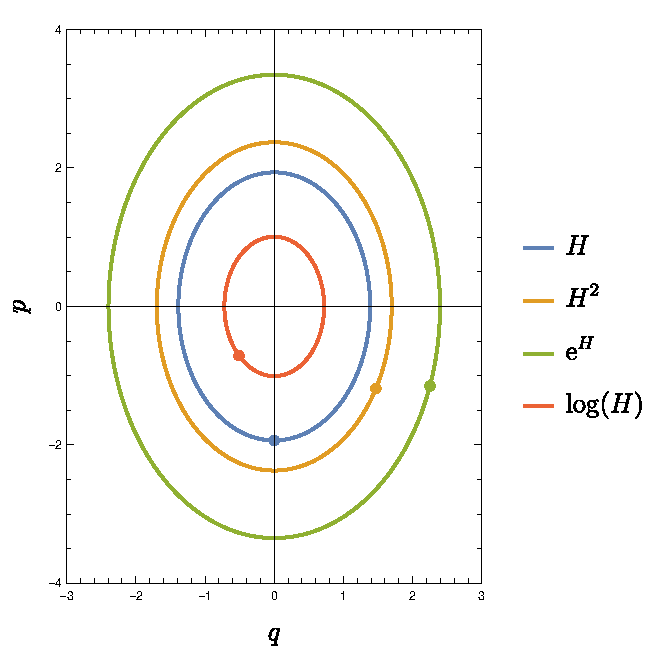
\includegraphics[width=0.4\textwidth]{Hreparam.pdf}
    \caption{Phase space diagram of the 1-dimensional harmonic oscillator in the $(q,p)$-plane for different $H$-reparametrizations shown in the legend of the plot. The points represent the values of $(q,p)$ at $t = 0$ which are shifted due to the non-trivial transformation of $T_0$ according to Eq.~\eqref{eq:H reparam: T0}.  The parameter values $m=1$, $\omega = 1.25$, $H = 1.5$ and $T_0 = 2\pi/5$ have been chosen for demonstrational purposes.}
    \label{fig:H reparam}
\end{figure}

We observed in the previous section that $T_0$-reparametrizations, $\tilde{T}_0 = \psi(T_0)$ cannot be understood as simple time reparametrizations as the new Hamiltonian attains an explicit time dependence for non-linear $\psi$. Still, ellipses in phase space are mapped to ellipses of different radii which now depends on the value of $H$ as well as on the value of initial time $T_0$. A visualization for various maps $\psi$ is given in Fig.~\ref{fig:T0 reparam}.

\begin{figure}
    \centering
    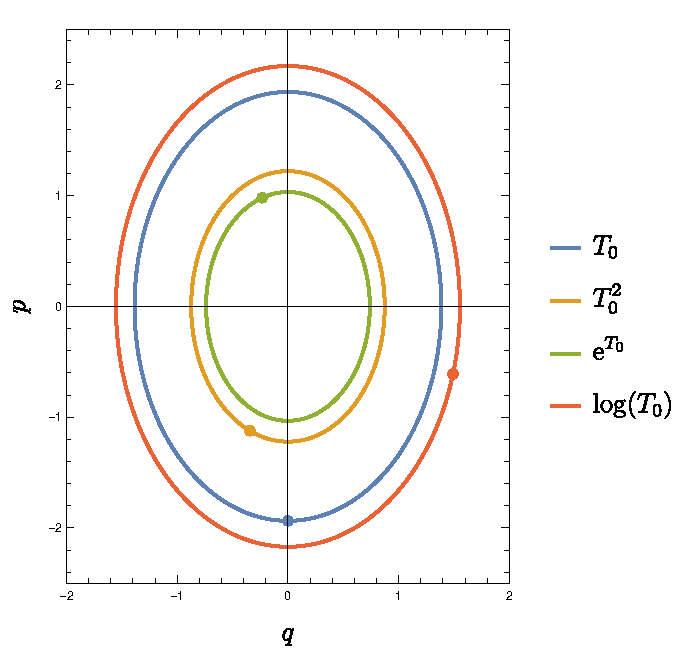
\includegraphics[width=0.4\textwidth]{T0reparam.pdf}
    \caption{Phase space diagram of the 1-dimensional harmonic oscillator in the $(q,p)$-plane for different $T_0$-reparametrizations shown in the legend of the plot. The points represent the values of $(q,p)$ at $t = 0$ which are shifted according to the map $\psi(T_0)$. The parameter values $m=1$, $\omega = 1.25$, $H = 1.5$ and $T_0 = 2\pi/5$ have been chosen for demonstrational purposes.}
    \label{fig:T0 reparam}
\end{figure}

The example of the single 1-dimensional harmonic oscillator can be straightforwardly generalized to d dimensions. That is because the Hamiltonian of the d-dimensional harmonic oscillator, given by 
%
\begin{equation}
H = \sum_{\alpha = 1}^\mathrm{d}\left(\frac{1}{2m}q_\alpha^2+\frac{m\omega^2}{2}q_\alpha^2\right),
\end{equation}
%
admits an immediate split into d 1-dimensional decoupled harmonic oscillators. As a result, the constants of motion $T_0^{(\alpha)}$ and $H^{(\alpha)}$ can be identified in analogy to Eq.~\eqref{eq:1D HO H and T0}. In the following section, we consider the example of coupled harmonic oscillators where this strategy cannot be directly applied due to the interaction term.


\section{Generally covariant quantum mechanics}

\subsection{Standard quantum harmonic oscillator}

Rewrite the standard quantum theory of the harmonic oscillator,
\be
[a, a^{\dagger}] = i \hbar,
\ee
with
\be
H = \hbar \omega \left( a^\dagger a + \frac{1}{2}\right) 
\ee
with  and vacuum state
\be
a |0 \ra = 0.
\ee
The operator $T_0$ cannot be expressed in terms of the creation and annihilation operators as it is an involved non-polynomial function of the classical canonical variables $(q,p)$. However, in close analogy to the action-angle variables developed in~\cite{Augustin1979}, one can introduce the operator $\hat{\tilde{H}}$  with eigenstates 
\be
\hat{\tilde{H}}\ket{n} = \hbar\omega\left(\hat{n}+\frac{1}{2}\right)\ket{n}, \quad n\in\mathbb{Z},
\ee
and its conjugate angle operator $\hat{\phi} = \omega \hat{T}_0$ with eigenstates
\be
\hat{\phi} \ket{\phi} = \phi \ket{\phi},
\ee
satisfying the canonical commutation relation
\be
[\hat{\phi},\hat{\tilde{H}}/\omega] = i \hbar.
\ee
Crucially, the spectrum of $\hat{\tilde{H}}$ is positive and negative. The states $\ket{\phi}$ are angles, $\ket{\phi = \phi+2\pi\mathbb{Z}}$, and the plane waves are given by $\braket{\phi}{n} = (2\pi)^{-1/2}\mathrm{e}^{i\phi n}$ on the unit circle $S^1$. To project onto the positive energy space, one needs to define the operator
\be
\hat{P} = \sum_{n = 0}^{\infty}\ket{n}\bra{n},
\ee
so that $\hat{H} = \hat{P}\hat{\tilde{H}}\hat{P}$.




\subsection{Hawking-like radiation in mechanics}

It is now interesting to compare the quantum description of the harmonic oscillator when performing a diffeomorphism 
\be
(H, T_0) \rightarrow  (\tilde{H}, \tilde{T}_0)
\ee
The novel result of this work is precisely that one has access to operator which switch from one description to another equivalent one. The interesting point here is that there is no preferred parameterization, i.e. coordinates of the space of motion. One can recover the situation familiar to QFT in curved spacetime: one is free to decompose the "field" to be quantize on different basis. Performing a change of parametrization of the space of motion should generate bogolioubov transformation and modify the number of particles seen by different observers associated to different parametrizations of the space of motion.

A special case would corresponds to the comparison between two parametrizations of the form
\be
\tilde{T}_0 = e^{\kappa T_0}
\ee
We know that this relation effectively introduce a partition of the real line which plays the role of an horizon. It is known that this partition naturally relates the vacuum seen in $\tilde{T}_0$ to a thermal vacuum  seen by $T_0$. See \cite{Arzano:2018oby,Arzano:2020mhg}. Using the same method, we have to show that i) the vacuum state is only relative to a given choice of $T_0$ and $H$, making explicit the notion of relative state in quantum mechanics, and ii) that one can reproduce the very same Hawking-like radiation and notion of temperature already in this generally covariant version of quantum mechanics. 




\section{Conclusion}

 \bigskip 

\noindent\textit{\textbf{Acknowledgements.}}
The authors thank Federico Capone, ... for helpful discussions. A. Jercher acknowledges support by the DFG under Grant No 406116891 within the Research Training Group RTG 2522/1 and under Grant No 422809950. The work of J. Ben Achour and A. Jercher is supported by the Munich Center for Quantum Science and Technology via the seed funding Aost 862981-8 granted by the DFG under Germany’s Excellence Strategy – EXC-2111 – 390814868 and by the Sir John Templeton fellowship.


\newpage
\appendix

\section{Hamilton-Jacobi method}

\label{HJM}

In this appendix, we recall the basic procedure to construct canonical cyclic variables through the Hamilton-Jacobi procedure. 
Consider an hamiltonian system with canonical variables $(q,p)$ and hamiltonian $H(q,p)$ which is not explicitly time-dependent such that
\be
\{ q, p\} =1\;, \qquad H(q,p) =E
\ee 
where $E$ is the energy of the system. 
The action of the system reads
\be
\label{action0}
\S = \int p \dd q - H \dd t
\ee
For such non dissipative one dimensional mechanical system, there is unique set of canonical variables which are cyclic, i.e. which correspond to canonically conjugated evolving constants of motion. We shall denote them $T_0$ and $E$. There are obtained through the Hamilton-Jacobi procedure. Consider the generating function $S(q, T_0, t)$ associated to the canonical transformation $(q,p) \rightarrow (T_0,E)$. The momenta satisfy
\be
p = \frac{\partial S(q,E, t)}{\partial q} \;, \qquad T_0 = - \frac{\partial S(q, E, t)}{\partial E} \;, 
\ee
By construction, the generating function $S(q, E, t)$ satisfies the Hamilton-Jacobi equation
\be
H_{\text{cycl}}(E, T_0, t) %= H(q, p) + \frac{\partial S(q, Q, t)}{\partial t} 
= H \left( q, \frac{\partial S}{\partial q} \right) + \frac{\partial S}{\partial t} = 0
\ee 
such that the new hamiltonian $H_{\text{cycl}}(E,T_0,t)$ vanishes identically. Consequently, the hamilton dynamics of the cyclic variables is given by
\be
\dot{E} = \frac{\partial H_{\text{cycl}}}{\partial T_0} = 0 \;, \qquad \dot{T}_0 = - \frac{\partial H_{\text{cycl}}}{\partial E} =0
\ee 
showing that these canonical variables are indeed constant of motion. These canonical variables $(T_0, E)$ provide therefore a parametrization of the two initial conditions $\left( q(0), \dot{q}(0)\right)$ for this 1d mechanical system as well as the associated physical trajectories on phase space. 

For mechanical system in which the hamiltonian is time-independent, it is customary to look for a solution of the generating function $S(q, E, t)$ by assuming the ansatz $S(q,E, t) = W(q,E) - E t$ where $W(q,E)$ is called the hamiltonian principal function. With this usual ansatz, one obtains
\begin{align}
E(q, p) & = W^{-1} (q, p) \;,\\
\label{P}
T_0(t,q, p) & = t - \frac{\partial W(q, E)}{\partial E}  \;.
\end{align}
Using that $T_0(t,q,p)$ is, by construction, a constant of motion, one has
\be
 \{T_0, E \} = \frac{\dd T_0}{\dd t} - \frac{\partial T_0}{\partial t} = 1
 \ee
 such that $(T_0, E)$ are canonically conjugated.
Provided the inverse of the function $W$ exists, one obtains the explicit expression of the cyclic variables $(T_0, E)$ in term of $(q,p, t)$. Notice that the conjugated cyclic momenta $T_0$ can be interpreted as the initial condition of the time coordinate.

\section{Generalization beyond 1d system}\label{sec:Extension}

The Hamilton-Jacobi formalism is applicable also to systems of multiple particles $N$ in higher dimensions $\mathrm{d}$ with the phase space thus being $2\mathrm{d}N$-dimensional. Consequently, the constants of motion $T_0^{(I)},H^{(I)}$ can be identified with $I\in\{1,\dots, 2\mathrm{d}N\}$ and the action taking the form
%
\begin{equation}
S[T_0^{(I)},H^{(I)}] = \sum_I\int H^{(I)}\dd{T_0^{(I)}}\, .
\end{equation}
%
Similar to the above, the generators of the Noether symmetry are given by
%
\begin{equation}
    W_{\vb*{m},\vb*{n}} = \prod_I \left(T_0^{(I)}\right)^{m_I+1}\left(H^{(I)}\right)^{n_I+1}\, , 
\end{equation}
%
with integers $(\vb*{m},\vb*{n})\in\mathbb{Z}^{2\mathrm{d}N}$. The algebra of these generators can be computed directly, yielding
%
\begin{equation}
\text{length expression but simple to compute}
\end{equation}
%
\textcolor{red}{To which algebra does this relate? Tensor product of Witt algebras?}

\subsection{ An example of a 2d system: the coupled harmonic oscillators}\label{sec:coupled HOs}

In this section, we study the interacting 1-dimensional mechanical system of two coupled harmonic oscillators, providing an example for the hidden Noether symmetry present in systems with more than one degree of freedom as discussed in Sec.~\ref{sec:Extension}. 

The Hamiltonian of two coupled harmonic oscillators is given by
%
\begin{equation}
H = \frac{1}{2m}\left(p_1^2+p_2^2\right)+\frac{k}{2}\left(q_1^2+q_2^2\right)+\frac{k_{12}}{2}(q_1-q_2)^2\, ,
\end{equation}
%
where we assume for simplicity that the masses as well as two of the three couplings $k$ are equal. The equations of motion are solved by
%
\begin{subequations}
\begin{align}
    q_1(t)&=\frac{1}{2}\left[A_1\cos(\omega_1 t+\phi_1)+A_2\cos(\omega_2 t+\phi_2)\right]\,, \\[7pt]
    q_2(t)&=\frac{1}{2}\left[A_1\cos(\omega_1 t+\phi_1)-A_2\cos(\omega_2 t+\phi_2)\right]\,,
\end{align}
\end{subequations}
%
with the momenta correspondingly obtained as $p_i = m\dot{q}_i$. The frequencies $\omega_1$ and $\omega_2$ are given in terms of $m,k$ and $k_{12}$ as
%
\begin{equation}
\omega_1 = \sqrt{\frac{k}{m}},\qquad \omega_2 = \sqrt{\frac{k+2k_{12}}{m}}
\end{equation}
%
In the present case of two harmonic oscillators, there are in total four initial conditions given by the constants $A_1,A_2,\phi_1$ and $\phi_2$. These constants coordinatize the space of motions.

As a consequence of the interaction term $\frac{k_{12}}{2}(q_1-q_2)^2$, the Hamiltonian does not admit an immediate split $H = H^{(1)}(q_1,p_1)+H^{(2)}(q_2,p_2)$. Thus, one cannot straightforwardly proceed as in the previous section and identify phase space functions $H^{(i)},T_0^{(i)}$ that relate to the constants $A_i,\phi_i$. Instead, we first perform a canonical transformation
%
\begin{subequations}
\begin{align}
  Q_1 = \frac{q_1+q_2}{2},\qquad & Q_2 = \frac{q_1-q_2}{2}\,,\\[7pt]
P_1 = p_1+p_2,\qquad & P_2 = p_1-p_2\,.  
\end{align}
\end{subequations}
%
such that the new Hamiltonian does not contain interactions between the two particles,
%
\begin{equation}
H(\{Q_i,P_i\}) = \frac{1}{m}\left(P_1^2+P_2^2\right)+kQ_1^2 + (k+2k_{12})Q_2^2\, , 
\end{equation}
%
thus allowing for a split $H = H^{(1)}(Q_1,P_1)+H^{(2)}(Q_2,P_2)$. 

Now, the analysis of the single harmonic oscillator of the previous section can be performed for the two particles individually and we identify
%
\begin{subequations}
\begin{align}
H^{(i)} &= \frac{1}{m}P_i^2+m\omega_i^2Q_i^2 = \frac{1}{4}m\omega_i^2A_i^2\, \\[7pt]
T_0^{(i)} &= -t-\frac{1}{\omega_i}\arctan\frac{P_i}{2m\omega_iQ_i}\, .
\end{align}   
\end{subequations}
%
As one can easily verify, the transformation $(Q_i,P_i)\mapsto (T_0^{(i)},H^{(i)})$ constitutes a canonical transformation with action
%
\begin{equation}
S = \sum_{i=1}^2\int H^{(i)}\dd{T_0^{(i)}}\, .
\end{equation}
%

The computation presented here for two coupled 1-dimensional harmonic oscillators can be straightforwardly generalized to $N$ coupled oscillators in d dimensions. As mentioned in the previous example, extending to d dimensions is simply achieved by indexing the constants $T_0$ and $H$ with an additional index $\alpha\in\{1,\dots,\mathrm{d}\}$. For the $N$ coupled particles, one then needs to identify a canonical transformation mapping to $N$ decoupled harmonic oscillators in d dimensions. As a result, the constants of motion $T_0^{(i,\alpha)}$ and $H^{(i,\alpha)}$ can be identified.

\textcolor{red}{
\begin{itemize}
    \item what about symmetry charges
\end{itemize}
}



\allowdisplaybreaks


\let\oldaddcontentsline\addcontentsline% Store \addcontentsline
\renewcommand{\addcontentsline}[3]{}% Make \addcontentsline a no-op

\bibliography{references.bib} 

%\bibliographystyle{utphys} 
%\providecommand{\href}[2]{#2}\begingroup\raggedright\begin{thebibliography}{10}



%\end{thebibliography}\endgroup

\let\addcontentsline\oldaddcontentsline% Restore \addcontentsline

%\input{template_SM}

\end{document}

